\documentclass[twocolumn]{article}
\usepackage[margin=0.6in,columnsep=0.15in]{geometry}
\usepackage[utf8]{inputenc}
\usepackage{stix}
\usepackage[usenames,dvipsnames]{xcolor}
\usepackage[colorlinks,citecolor=Gray,urlcolor=Gray,linkcolor=Blue]{hyperref}
\usepackage[small]{titlesec}

\usepackage{authblk}
\renewcommand\Affilfont{\itshape\small} % chktex 6

\usepackage[normal]{caption}
\DeclareCaptionLabelSeparator{pipe}{ $|$ }
\captionsetup{labelsep=pipe}
\renewcommand{\captionfont}{\small}
\renewcommand{\captionlabelfont}{\bfseries}

\usepackage[sort&compress]{natbib}
\bibliographystyle{abbrvnat}
\renewcommand\cite{\citep}
\usepackage{doi}

\usepackage{graphicx}
\usepackage{mathtools}
\usepackage{booktabs}
\usepackage{tabularx}
\usepackage{tikz}

\usepackage[export]{adjustbox}
\title{\input{title.txt}\\(Supplementary information)}

\author[1,2]{Jan Hermann}
\author[2,*]{Alexandre Tkatchenko}
\affil[1]{Fritz-Haber-Institut der Max-Planck-Gesellschaft, Faradayweg 4--6, 14195 Berlin, Germany}
\affil[2]{Physics and Materials Science Research Unit, University of Luxembourg, 162A Avenue de la Faïencerie, L-1511 Luxembourg}

\date{}

\setcounter{secnumdepth}{0}

\begin{document}

\nocite{achemso-control}

\maketitle

\begingroup
\renewcommand\thefootnote{}\footnote{$^*$Email: alexandre.tkatchenko@uni.lu}%
\addtocounter{footnote}{-1}%
\endgroup
All resources for the manuscript, including the manuscript itself, can be found in a Git repository~\cite{GitRepo} and related data files~\cite{DataH5,DataCaf}.
This includes scripts used to generate input files, all inputs and output files, data processing scripts, data, figures, and \LaTeX\ source files.
The file organization is described in \verb+/README.md+, while here, we summarize the scientifically relevant information and present additional analysis of the data.

The performed calculations comprise:
(i) DFT and van der Waals (vdW) calculations on benchmark sets 3B-69, L7, S12L, S22, S66, X40, X23, and on rare-gas dimers and additional supramolecular complexes, both with standard semi-local functionals (\verb+/calc/2017-01-23-all-vdw-sets-3+) as well as the modified SCAN functional (\verb+/calc/2017-04-24-scan-modifications+);
(ii) DFT calculations on the graphene-flake dimers (\verb+/calc/2017-02-13-graphene-flakes+).
All DFT calculations were done with FHI-aims~\cite{BlumCPC09}, which uses atom-centered basis sets with numerical radial parts.
We used the \verb+tight+ default basis set and grid settings, which ensure numerical convergence to 0.1\,kcal/mol in binding energies for the van der Waals (vdW) systems studied here.

The VV10 nonlocal functional (its rVV10 variant~\cite{SabatiniPRB13}) was evaluated with Quantum Espresso~\cite{GiannozziJPCM09} and norm-conserving Vanderbilt pseudopotentials~\cite{HamannPRB13}.
Quantum Espresso uses plane-wave basis sets, and so is restricted to periodic boundary conditions only.
To calculate the binding energies of isolated molecular systems, we used the plane-wave cutoff of 30\,Ry, and separated the periodic images with 8\,\AA\ of vacuum, which converges vdW binding energies to 0.1\,kcal/mol (Figure~\ref{fig:bz-tests-padding-basis}, \verb+/calc/2017-03-24-benzene-dimer-qe-tests+).

\begin{figure*}
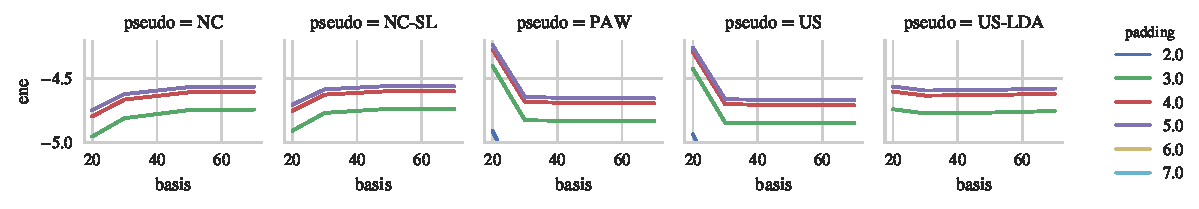
\includegraphics[center]{media/bz-tests-padding-basis}
\caption{\textbf{Label.}
Text.
}\label{fig:bz-tests-padding-basis}
\end{figure*}

For crystals, $k$-point grids with density of at least 0.8\,\AA\ in reciprocal space were used for all DFT, MBD, and VV10 calculations.

Both VV10 and MBD depend on the electron density, and in principle should be calculated for each density functional separately, but in practice the differences between the densities from different functionals are of the sort that changes the vdW energies only negligibly.
Therefore, we calculated MBD on PBE densities, and VV10 on the originally suggested combination of reparameterized PW86 exchange and PBE correlation.

All molecular crystal geometries were taken directly from the respective benchmark sets without any relaxation and can be obtained directly from the repository or as supplementary data.

\begin{figure*}
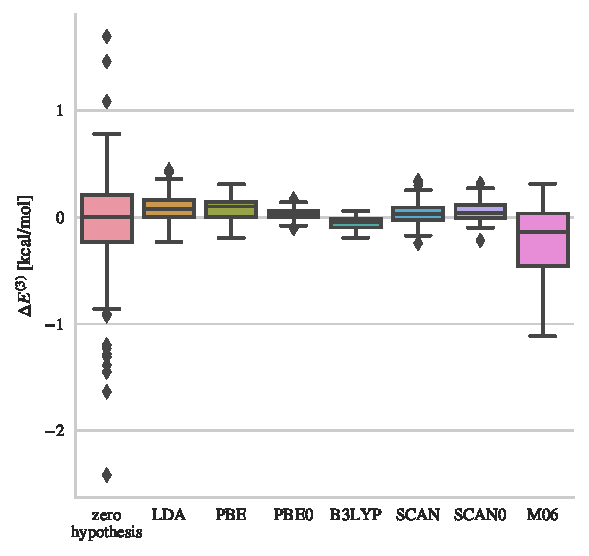
\includegraphics[center]{media/3-body}
\caption{\textbf{Distributions of relative errors in 3-body interaction energies on the 3B-69 set.}
The box-and-whisker plot is of the same kind as Figure~1 in the main text.
The ``zero hypothesis'' corresponds to a method which always gives zero 3-body interaction energy.
}\label{fig:3-body}
\end{figure*}

\begin{figure*}
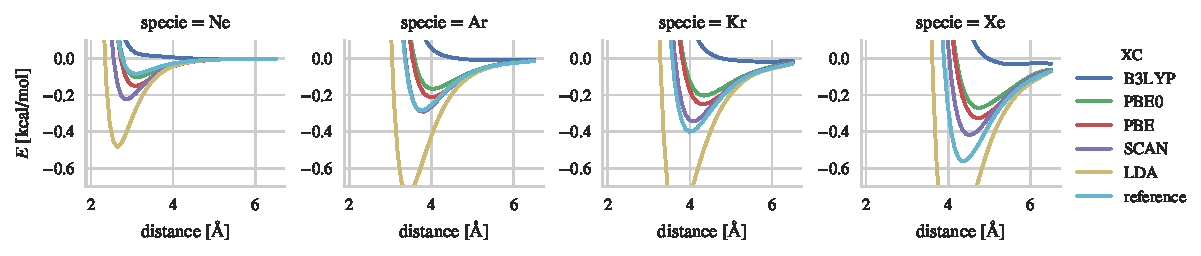
\includegraphics[center]{media/mbd-rare-gas}
\caption{\textbf{Binding curves of rare-gas dimers.}
The reference is a highly accurate empirical potential parametrized on experimental data.
}\label{fig:mbd-rare-gas}
\end{figure*}

\begin{figure*}
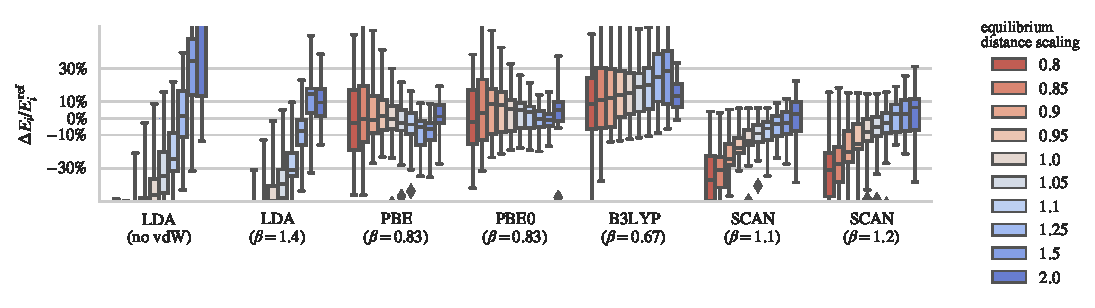
\includegraphics[center]{media/x40-dists}
\caption{\textbf{Distributions of relative errors in binding energies on the  X40 set of several DFT+MBD combinations.}
}\label{fig:x40-dists}
This is an equivalent of Figure~1 from the main text for the X40 set.
\end{figure*}

\begin{figure*}
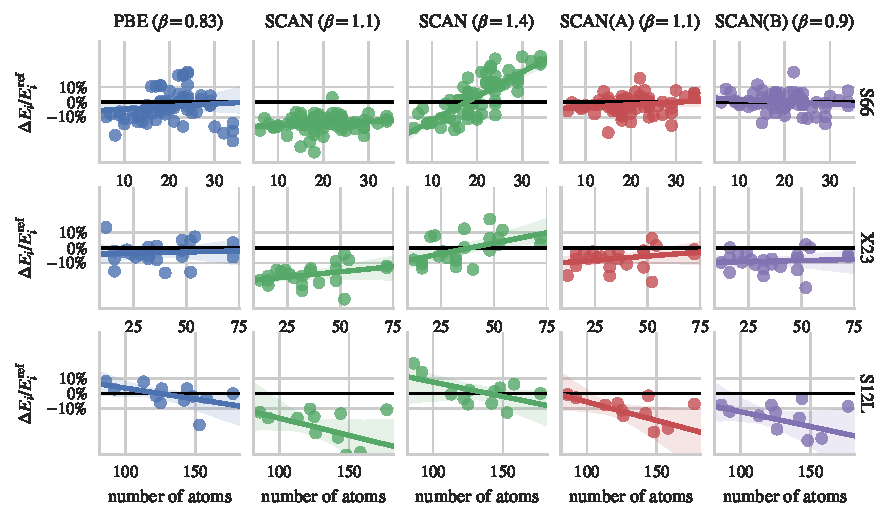
\includegraphics[center]{media/size-dependence}
\caption{\textbf{Dependence of relative errors in binding energies on system size of several DFT+MBD combinations.}
}\label{fig:size-dependence}
\end{figure*}

\begin{figure*}
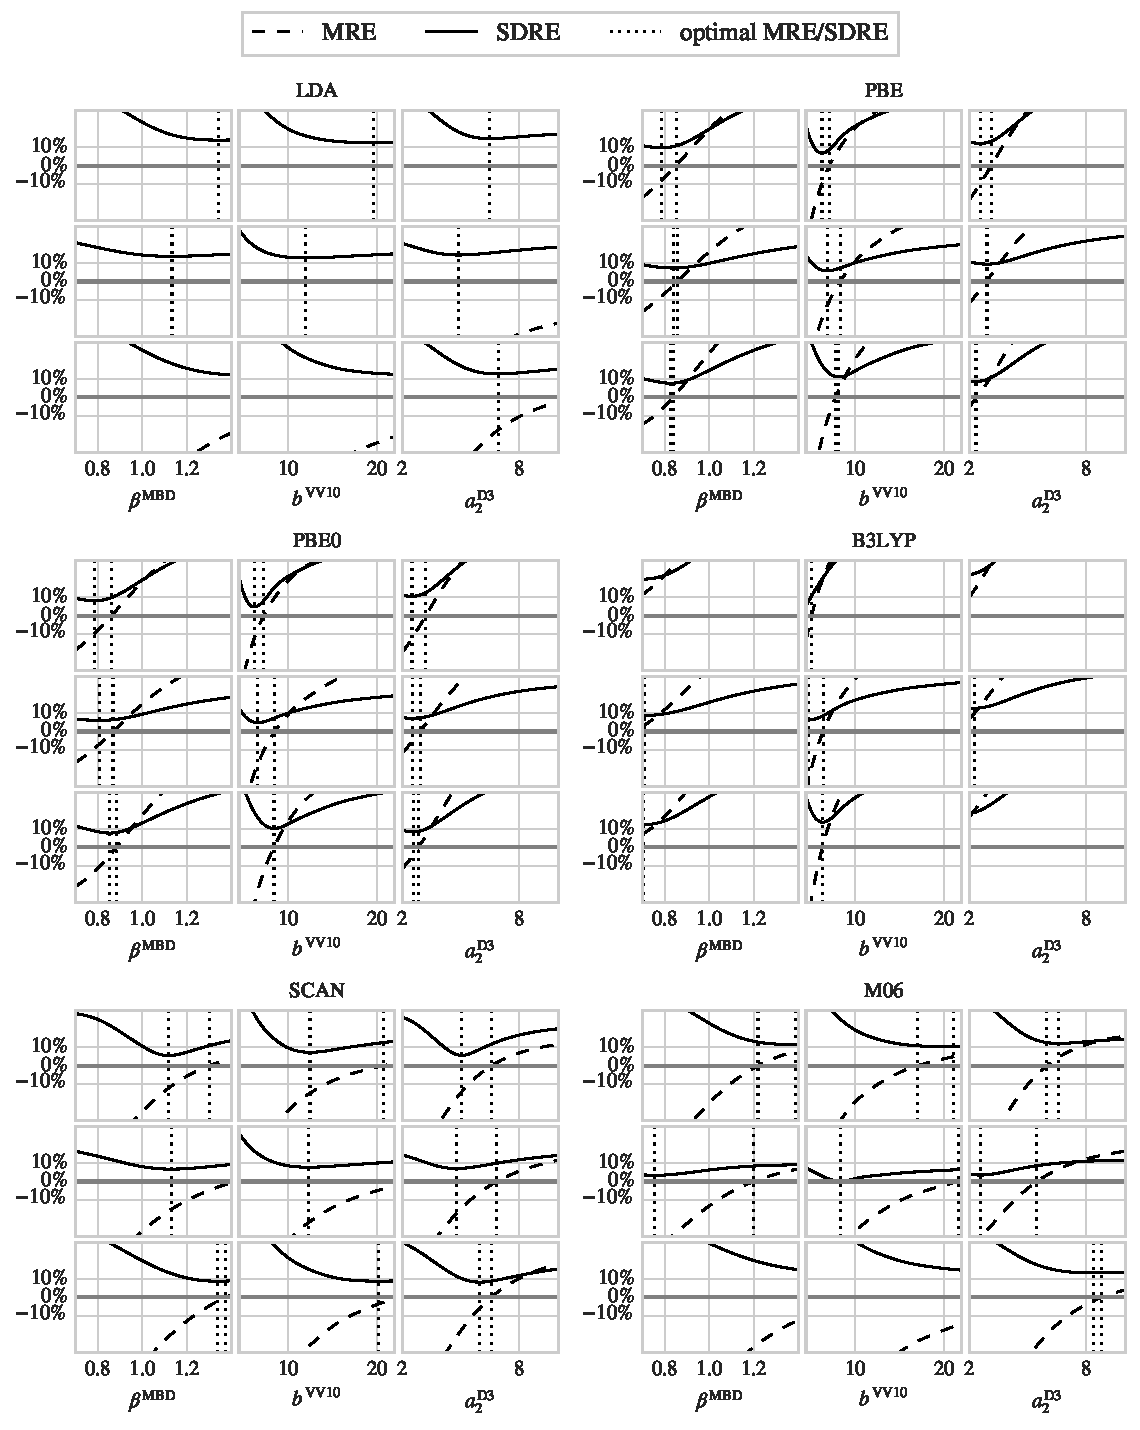
\includegraphics[center]{media/param-fitting-all}
\caption{\textbf{Dependence of means (MRE) and standard deviations (SDRE) of relative errors in binding energies on range-separation parameters.}
This is an extension of Figure~2 from the main text to all semi-local functionals.
}\label{fig:param-fitting-all}
\end{figure*}

\section{Supplementary results}

Figure~\ref{fig:3-body} shows the errors of density functionals in 3-body interaction energies calculated on the 3B-69 set~\cite{RezacJCTC15}.
Figure~\ref{fig:mbd-rare-gas} shows the interaction curves of rare-gas dimers calculated with different density functionals.
Figure~\ref{fig:x40-dists} shows the error distributions on the X40 set.
Figure~\ref{fig:size-dependence} shows the dependence of relative errors on system size.
Figure~\ref{fig:param-fitting-all} is the extension of Figure~2 from the main text to all density functionals.

\begingroup
\renewcommand{\section}[2]{}
\setlength\bibsep{0pt}
\footnotesize
\bibliography{refs-zotero,refs}
\endgroup

\end{document}
